% Options for packages loaded elsewhere
\PassOptionsToPackage{unicode}{hyperref}
\PassOptionsToPackage{hyphens}{url}
%
\documentclass[
]{article}
\usepackage{lmodern}
\usepackage{amssymb,amsmath}
\usepackage{ifxetex,ifluatex}
\ifnum 0\ifxetex 1\fi\ifluatex 1\fi=0 % if pdftex
  \usepackage[T1]{fontenc}
  \usepackage[utf8]{inputenc}
  \usepackage{textcomp} % provide euro and other symbols
\else % if luatex or xetex
  \usepackage{unicode-math}
  \defaultfontfeatures{Scale=MatchLowercase}
  \defaultfontfeatures[\rmfamily]{Ligatures=TeX,Scale=1}
\fi
% Use upquote if available, for straight quotes in verbatim environments
\IfFileExists{upquote.sty}{\usepackage{upquote}}{}
\IfFileExists{microtype.sty}{% use microtype if available
  \usepackage[]{microtype}
  \UseMicrotypeSet[protrusion]{basicmath} % disable protrusion for tt fonts
}{}
\makeatletter
\@ifundefined{KOMAClassName}{% if non-KOMA class
  \IfFileExists{parskip.sty}{%
    \usepackage{parskip}
  }{% else
    \setlength{\parindent}{0pt}
    \setlength{\parskip}{6pt plus 2pt minus 1pt}}
}{% if KOMA class
  \KOMAoptions{parskip=half}}
\makeatother
\usepackage{xcolor}
\IfFileExists{xurl.sty}{\usepackage{xurl}}{} % add URL line breaks if available
\IfFileExists{bookmark.sty}{\usepackage{bookmark}}{\usepackage{hyperref}}
\hypersetup{
  pdftitle={MStractor Workflow},
  pdfauthor={Luca Nicolotti, The Australian Wine Research Institute, Metabolomics Australia},
  hidelinks,
  pdfcreator={LaTeX via pandoc}}
\urlstyle{same} % disable monospaced font for URLs
\usepackage[margin=1in]{geometry}
\usepackage{color}
\usepackage{fancyvrb}
\newcommand{\VerbBar}{|}
\newcommand{\VERB}{\Verb[commandchars=\\\{\}]}
\DefineVerbatimEnvironment{Highlighting}{Verbatim}{commandchars=\\\{\}}
% Add ',fontsize=\small' for more characters per line
\usepackage{framed}
\definecolor{shadecolor}{RGB}{248,248,248}
\newenvironment{Shaded}{\begin{snugshade}}{\end{snugshade}}
\newcommand{\AlertTok}[1]{\textcolor[rgb]{0.94,0.16,0.16}{#1}}
\newcommand{\AnnotationTok}[1]{\textcolor[rgb]{0.56,0.35,0.01}{\textbf{\textit{#1}}}}
\newcommand{\AttributeTok}[1]{\textcolor[rgb]{0.77,0.63,0.00}{#1}}
\newcommand{\BaseNTok}[1]{\textcolor[rgb]{0.00,0.00,0.81}{#1}}
\newcommand{\BuiltInTok}[1]{#1}
\newcommand{\CharTok}[1]{\textcolor[rgb]{0.31,0.60,0.02}{#1}}
\newcommand{\CommentTok}[1]{\textcolor[rgb]{0.56,0.35,0.01}{\textit{#1}}}
\newcommand{\CommentVarTok}[1]{\textcolor[rgb]{0.56,0.35,0.01}{\textbf{\textit{#1}}}}
\newcommand{\ConstantTok}[1]{\textcolor[rgb]{0.00,0.00,0.00}{#1}}
\newcommand{\ControlFlowTok}[1]{\textcolor[rgb]{0.13,0.29,0.53}{\textbf{#1}}}
\newcommand{\DataTypeTok}[1]{\textcolor[rgb]{0.13,0.29,0.53}{#1}}
\newcommand{\DecValTok}[1]{\textcolor[rgb]{0.00,0.00,0.81}{#1}}
\newcommand{\DocumentationTok}[1]{\textcolor[rgb]{0.56,0.35,0.01}{\textbf{\textit{#1}}}}
\newcommand{\ErrorTok}[1]{\textcolor[rgb]{0.64,0.00,0.00}{\textbf{#1}}}
\newcommand{\ExtensionTok}[1]{#1}
\newcommand{\FloatTok}[1]{\textcolor[rgb]{0.00,0.00,0.81}{#1}}
\newcommand{\FunctionTok}[1]{\textcolor[rgb]{0.00,0.00,0.00}{#1}}
\newcommand{\ImportTok}[1]{#1}
\newcommand{\InformationTok}[1]{\textcolor[rgb]{0.56,0.35,0.01}{\textbf{\textit{#1}}}}
\newcommand{\KeywordTok}[1]{\textcolor[rgb]{0.13,0.29,0.53}{\textbf{#1}}}
\newcommand{\NormalTok}[1]{#1}
\newcommand{\OperatorTok}[1]{\textcolor[rgb]{0.81,0.36,0.00}{\textbf{#1}}}
\newcommand{\OtherTok}[1]{\textcolor[rgb]{0.56,0.35,0.01}{#1}}
\newcommand{\PreprocessorTok}[1]{\textcolor[rgb]{0.56,0.35,0.01}{\textit{#1}}}
\newcommand{\RegionMarkerTok}[1]{#1}
\newcommand{\SpecialCharTok}[1]{\textcolor[rgb]{0.00,0.00,0.00}{#1}}
\newcommand{\SpecialStringTok}[1]{\textcolor[rgb]{0.31,0.60,0.02}{#1}}
\newcommand{\StringTok}[1]{\textcolor[rgb]{0.31,0.60,0.02}{#1}}
\newcommand{\VariableTok}[1]{\textcolor[rgb]{0.00,0.00,0.00}{#1}}
\newcommand{\VerbatimStringTok}[1]{\textcolor[rgb]{0.31,0.60,0.02}{#1}}
\newcommand{\WarningTok}[1]{\textcolor[rgb]{0.56,0.35,0.01}{\textbf{\textit{#1}}}}
\usepackage{graphicx}
\makeatletter
\def\maxwidth{\ifdim\Gin@nat@width>\linewidth\linewidth\else\Gin@nat@width\fi}
\def\maxheight{\ifdim\Gin@nat@height>\textheight\textheight\else\Gin@nat@height\fi}
\makeatother
% Scale images if necessary, so that they will not overflow the page
% margins by default, and it is still possible to overwrite the defaults
% using explicit options in \includegraphics[width, height, ...]{}
\setkeys{Gin}{width=\maxwidth,height=\maxheight,keepaspectratio}
% Set default figure placement to htbp
\makeatletter
\def\fps@figure{htbp}
\makeatother
\setlength{\emergencystretch}{3em} % prevent overfull lines
\providecommand{\tightlist}{%
  \setlength{\itemsep}{0pt}\setlength{\parskip}{0pt}}
\setcounter{secnumdepth}{-\maxdimen} % remove section numbering

\title{MStractor Workflow}
\author{Luca Nicolotti, The Australian Wine Research Institute,
Metabolomics Australia}
\date{26/02/2020}

\begin{document}
\maketitle

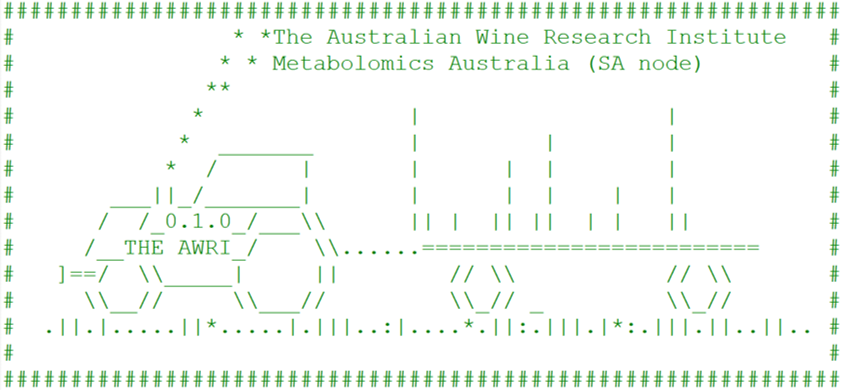
\includegraphics{./vignettespicture.png}

\hypertarget{introduction}{%
\subsection{\texorpdfstring{\emph{Introduction}}{Introduction}}\label{introduction}}

\textbf{MStractor} combines the functions for molecular feature
extraction present in XCMS and CAMERA with user friendly dedicated GUIs
for LC and MS parameters input, graphical QC outputs and descriptive
statistics calculation.

A schematic representation of the workflow is displayed in
\textbf{Figure 1}, reported below. The workflow consists of 10 steps
with the possibility of running the workflow using either the most
recent xcms functions specific for \emph{XCMSnExp} objects
(\textbf{branch a}) or the old set of functions for \emph{xcmsSet}
objects (\textbf{branch b}). However, the 2 branches perform the same
data processing steps and produce similar outputs. The reason of
developing 2 parallel frameworks mainly depends on the availability of
computational power on the user's end. Specifically, authors observed
that step \textbf{6a} tends to be quite time-consuming in particular
when dealing with complex datasets. Therefore, in case of limited
computing resources and large datasets, the authors suggest using branch
b of the workflow. The 2 frameworks merge at step 8, where the data set
is processed using CAMERA. Since the latest release available for CAMERA
does not support XCMSnEXP objects, the data set object is required to be
converted to the xcmsSet format prior to this step.

\begin{center}\rule{0.5\linewidth}{0.5pt}\end{center}

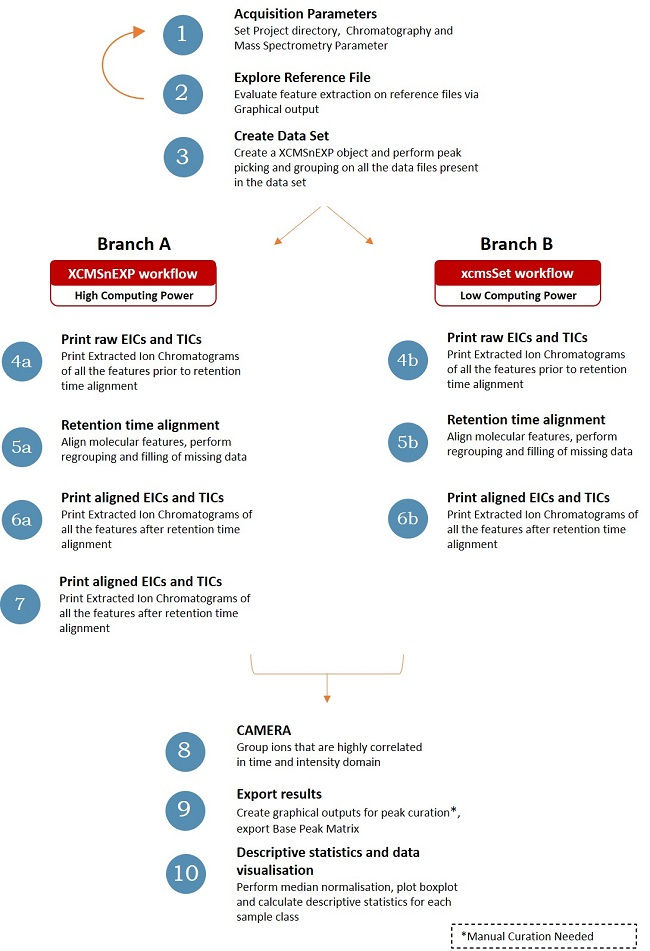
\includegraphics{./workflow.jpg} \textbf{Figure 1} = `Schematic
representation of MStractor Workflow'

\begin{center}\rule{0.5\linewidth}{0.5pt}\end{center}

Each step of the framework displayed in Figure 1 involves using 1 or
more functions. MStractor functions can be classified into 3 different
groups:

\textbf{1.MStractor specific functions}: developed by the authors to
provide the user with a friendly and seamless experience. The functions
belonging to this class mainly involve the use of GUIs allowing
parameters input and storage to be used later in the workflow. This
calss also include functions to normalise data and calculate basic
statistics.

\textbf{2.Wrapper functions}: this category includes wrapper functions
of xcms and CAMERA. The function backbone is the xcms (or CAMERA)
function and additional code is used to automate routine operations and
produce graphical outputs within the selected working directory.

\textbf{3.xcms and CAMERA functions}: these functions are basic CAMERA
and xcms function that are used along the workflow. However, the user is
not required to update the function arguments because all the necessary
parameters are input in the previous steps of the workflow

\hypertarget{data-preparation-and-file-naming}{%
\subsection{\texorpdfstring{\emph{Data Preparation and File
Naming}}{Data Preparation and File Naming}}\label{data-preparation-and-file-naming}}

Preparing the data and creating the correct working directory and folder
structure (outside the R environment) is required prior to executing the
workflow. The raw data files need to be converted to an appropriate
format which can be easily achieved using various tools freely
available, such as Proteowizard (ProteWizard,
\url{http://proteowizard.sourceforge.net/}) and Massmatrix (MassMatrix,
\url{http://www.massmatrix.net/}). MStractor supported file formats
include CDF, mzDATA, mzML and mzXML. After conversion, files should be
grouped in folders according to their class of belonging. Every
class-folder needs to be stored within the directory `MSfiles'. The
script will use the `MSfiles' subfolder downstream to automatically
determine the sample classes required for processing. If the folder
`MSfiles' is not present, the user will encounter errors. For each
class-folder a minimum of 2 replicates is required. An example dataset
(see Figure2) is provided with the package.

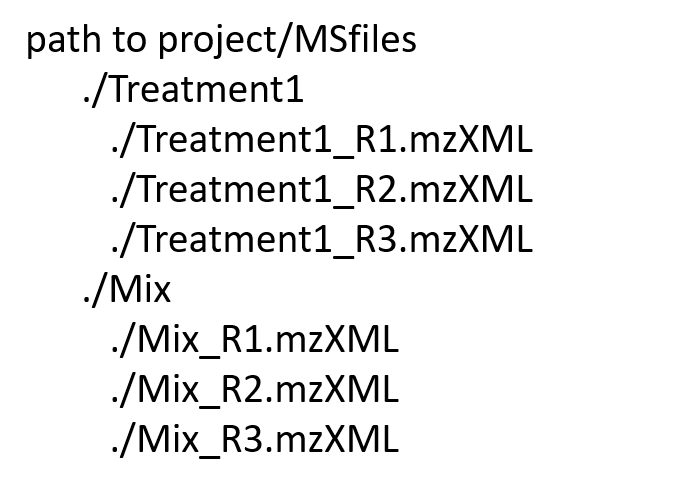
\includegraphics{./subdirchart.png}

\textbf{Figure 2} = `Project subfolder structure'

File naming is a key aspect for correct visualisation of graphical
output. This becasue a specific function of the workflow assigns
different colours and symbols to the different sample classes. In this
respect, the filename has to correspond to the folder name followed by
an underscore and a number inidicating the biological replicate, as
displayed in \textbf{Figure 2}.

\hypertarget{installation}{%
\subsection{\texorpdfstring{\emph{Installation
}}{Installation }}\label{installation}}

Download the tar.gz package from
\url{https://github.com/MetabolomicsSA/MStractor/releases} and run the
following (the setRepositories command allows downoading the required
dependencies from both the CRAN and Bioconductor) Define the tar.gz
location.

\begin{Shaded}
\begin{Highlighting}[]
\KeywordTok{setRepositories}\NormalTok{(}\DataTypeTok{ind=}\DecValTok{1}\OperatorTok{:}\DecValTok{2}\NormalTok{)}

\NormalTok{remotes}\OperatorTok{::}\KeywordTok{install\_local}\NormalTok{(}\StringTok{"C:/pathtoPackage/MStractor\_0.1.0.tar.gz"}\NormalTok{, }
 \StringTok{\textquotesingle{}               dependencies=NA)}
\end{Highlighting}
\end{Shaded}

\begin{Shaded}
\begin{Highlighting}[]
\KeywordTok{library}\NormalTok{(MStractor)}
\end{Highlighting}
\end{Shaded}

\hypertarget{acquisition-parameters}{%
\subsection{\texorpdfstring{1. \emph{Acquisition
Parameters}}{1. Acquisition Parameters}}\label{acquisition-parameters}}

The first step of the workflow consists in running 6 functions that
allow the input of chromatographic, mass spectrometry and peak picking
parameters as well as loading the data and automatically define the
visualization settings for graphical outputs.

The standard input values provided in each function are based on the
settings of the acquisition instrument used by the authors and,
therefore, suitable for processing the example data set available within
the package. These criteria should be changed according to the user's
LCMS system configuration, since they can dramatically influence the
data processing outcome.

\hypertarget{define-working-directory-and-reference-files}{%
\subsubsection{\texorpdfstring{1.1 \emph{Define Working Directory and
Reference
Files}}{1.1 Define Working Directory and Reference Files}}\label{define-working-directory-and-reference-files}}

\begin{Shaded}
\begin{Highlighting}[]
\KeywordTok{Project}\NormalTok{()}
\CommentTok{\#Skip this step if using the dataset provided within the package }
\end{Highlighting}
\end{Shaded}

use instead:

\begin{Shaded}
\begin{Highlighting}[]
\NormalTok{path<{-}}\KeywordTok{system.file}\NormalTok{(}\StringTok{"extdata"}\NormalTok{,}\DataTypeTok{package =} \StringTok{"MStractor"}\NormalTok{)}
\NormalTok{files <{-}}\StringTok{ }\KeywordTok{dir}\NormalTok{(path, }\DataTypeTok{pattern =} \StringTok{".mzXML"}\NormalTok{, }\DataTypeTok{full.names =} \OtherTok{TRUE}\NormalTok{)}
\end{Highlighting}
\end{Shaded}

The function doesn't require arguments. Its execution opens a GUI
(Figure 3) allowing the selection of the working directory and 2
reference fileschosen from one of the folders within the MSfiles
directory (e.g.: 2 `Mix' replicates in the example dataset). The
function also creates a QC folder where graphical outputs to evaluate
the progressing of the workflow are stored .

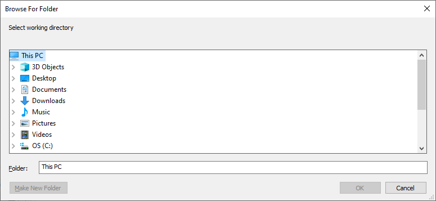
\includegraphics{./selectwd.png}

\textbf{Figure 3: GUI for project folder selection}

\hypertarget{input-of-chromatographic-and-mass-spectrometry-parameters}{%
\subsubsection{\texorpdfstring{1.2 \emph{Input of Chromatographic and
Mass Spectrometry
Parameters}}{1.2 Input of Chromatographic and Mass Spectrometry Parameters}}\label{input-of-chromatographic-and-mass-spectrometry-parameters}}

ChromParam() allows the user to input the chromatographic parameters
related to the data set to be processed and that will be stored and used
in the later stages of the framework. The values to be entered are the
retention time range of the data set (rt start and rt end), the maximum
retention time drift observed and the minimum and maximum fullwidth at
half maximun (FWHM min and max).

MassSpecParam() is mainly used to input mass spectrometry related
parameters. The criteria to be entered are the acquisition mode
(negative as default); the mass range to be considered (mz start and mz
end); the number of expected charges (default value set at 3); the file
type (default set to `.mzXML'); the maximum number of chromatographic
peaks expected for a single EIC and the sensitivity.

Both the functions return the input parameteres.

For more details about more details about the parameters consult the
xcms manual:
\url{https://www.bioconductor.org/packages/release/bioc/manuals/xcms/man/xcms.pdf}
)

\begin{Shaded}
\begin{Highlighting}[]
\KeywordTok{ChromParam}\NormalTok{()}
\end{Highlighting}
\end{Shaded}

\begin{verbatim}
## [[1]]
## [1] 1
## 
## [[2]]
## [1] "max"
## 
## [[3]]
## [1] 10
## 
## [[4]]
## [1] 90
## 
## [[5]]
## [1] 32
\end{verbatim}

\begin{Shaded}
\begin{Highlighting}[]
\KeywordTok{MassSpecParam}\NormalTok{()}
\end{Highlighting}
\end{Shaded}

\begin{verbatim}
## [[1]]
## [1] "negative"
## 
## [[2]]
## [1] 100
## 
## [[3]]
## [1] 1650
## 
## [[4]]
## [1] 0.01
## 
## [[5]]
## [1] 3
## 
## [[6]]
## [1] 30
## 
## [[7]]
## [1] 0.2
## 
## [[8]]
## [1] ".mzXML"
\end{verbatim}

\begin{Shaded}
\begin{Highlighting}[]
\CommentTok{\# leave default values if using the package dataset}
\end{Highlighting}
\end{Shaded}

Values are entered using GUIs as displayed in Figure 4.

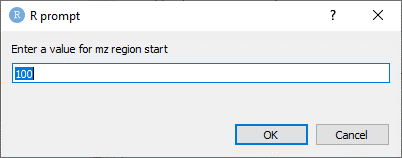
\includegraphics{./massspecparam.png}

\textbf{Figure 4: example of GUI input parameters}

\hypertarget{load-the-dataset}{%
\subsubsection{\texorpdfstring{1.3 \emph{Load the
Dataset}}{1.3 Load the Dataset}}\label{load-the-dataset}}

\begin{Shaded}
\begin{Highlighting}[]
\KeywordTok{LoadData}\NormalTok{()}
\CommentTok{\#Skip this step if using the dataset provided within the package }
\end{Highlighting}
\end{Shaded}

The function returns a complete list of the loaded files. It also starts
recording the time necessary for data processing and creates the object
`ClassType' which associates every data file with the class of
belonging.

\hypertarget{define-class-identifiers}{%
\subsubsection{\texorpdfstring{1.4 \emph{Define Class
Identifiers}}{1.4 Define Class Identifiers}}\label{define-class-identifiers}}

\begin{Shaded}
\begin{Highlighting}[]
\NormalTok{ClassType<{-}}\KeywordTok{c}\NormalTok{(}\StringTok{\textquotesingle{}Mix\textquotesingle{}}\NormalTok{,}\StringTok{\textquotesingle{}Treatment1\textquotesingle{}}\NormalTok{)}\CommentTok{\#\# use only with the provided dataset}
\KeywordTok{DefineClassAttributes}\NormalTok{(ClassType)}
\end{Highlighting}
\end{Shaded}

\begin{verbatim}
## [[1]]
## [1] "Mix"        "Mix"        "Mix"        "Treatment1" "Treatment1" "Treatment1"
## 
## [[2]]
## [1] "#FF0000FF" "#FF0000FF" "#FF0000FF" "#00FFFFFF" "#00FFFFFF" "#00FFFFFF"
## 
## [[3]]
## [1] 1 1 1 2 2 2
\end{verbatim}

The argument of the function is the object `ClassType'. The function
defines and returns specific symbols and colours for each sample class,
which are then used to produce graphical outputs.

\hypertarget{define-peak-picking-parameters}{%
\subsubsection{\texorpdfstring{1.5 \emph{Define Peak Picking
Parameters}}{1.5 Define Peak Picking Parameters}}\label{define-peak-picking-parameters}}

\begin{Shaded}
\begin{Highlighting}[]
\CommentTok{\#leave default values if using the package dataset}
\KeywordTok{PeakPickingParam}\NormalTok{()}
\end{Highlighting}
\end{Shaded}

\begin{verbatim}
## [[1]]
## [1] 10
## 
## [[2]]
## [1] 20
## 
## [[3]]
## [1] 3.030303
## 
## [[4]]
## [1] 50
## 
## [[5]]
## [1] 26.51515
## 
## [[6]]
## [1] 0.002
## 
## [[7]]
## [1] FALSE
## 
## [[8]]
## [1] 1
\end{verbatim}

The function uses GUIs to define xcms peak picking parameters using the
centwave algorithm. These include: minimum and maximum peakwidth,
minimum and maximum m/z error (in ppm), values for the integration
threshold (set at 5000) and signal to noise threshold, the integration
method to be used (1 or 2 as defined by the xcms documentation) and
whether the pick picking should fit the gaussian curve. The default
value for minimum and maximum m/z error and signal to noise (S/N)
threshold is `none' and correspond, respectively, to 3.03 and 50 ppm and
1000 for S/N value. Detailed information about the mentioned parameters
can be found in the xcms documentation
\url{https://www.bioconductor.org/packages/}
release/bioc/manuals/xcms/man/xcms.pdf

\hypertarget{parameter-evaluation}{%
\subsection{\texorpdfstring{2. \emph{Parameter
Evaluation}}{2. Parameter Evaluation}}\label{parameter-evaluation}}

This step allows testing the suitability of the input parameters on the
reference files selected in the first step.

\begin{Shaded}
\begin{Highlighting}[]
\KeywordTok{exploreRefs}\NormalTok{() }
\end{Highlighting}
\end{Shaded}

Note: In case the package dataset is used, the following needs to be run

\begin{Shaded}
\begin{Highlighting}[]
\KeywordTok{dir.create}\NormalTok{(}\StringTok{"./QC"}\NormalTok{)}
\NormalTok{SampleGroup<{-}}\KeywordTok{c}\NormalTok{(}\StringTok{"Mix"}\NormalTok{, }\StringTok{"Mix"}\NormalTok{)}
\NormalTok{symbol<{-}}\KeywordTok{c}\NormalTok{(}\DecValTok{1}\NormalTok{,}\DecValTok{1}\NormalTok{)}
\NormalTok{ClassCol<{-}}\KeywordTok{c}\NormalTok{(}\StringTok{"\#FF0000FF"}\NormalTok{, }\StringTok{"\#FF0000FF"}\NormalTok{)}
\NormalTok{path<{-}}\KeywordTok{system.file}\NormalTok{(}\StringTok{"extdata"}\NormalTok{,}\DataTypeTok{package =} \StringTok{"MStractor"}\NormalTok{)}
\NormalTok{files <{-}}\StringTok{ }\KeywordTok{dir}\NormalTok{(path, }\DataTypeTok{pattern =} \StringTok{".mzXML"}\NormalTok{, }\DataTypeTok{full.names =} \OtherTok{TRUE}\NormalTok{)}
\NormalTok{test<{-}files[}\DecValTok{1}\OperatorTok{:}\DecValTok{2}\NormalTok{]}
\NormalTok{pd <{-}}\StringTok{ }\KeywordTok{data.frame}\NormalTok{(}\DataTypeTok{sample\_name =} \KeywordTok{sub}\NormalTok{(}\KeywordTok{basename}\NormalTok{(test), }\DataTypeTok{pattern =}\NormalTok{ filetype,}
    \DataTypeTok{replacement =}\StringTok{""}\NormalTok{, }\DataTypeTok{fixed =} \OtherTok{TRUE}\NormalTok{),}\DataTypeTok{sample\_group =}\NormalTok{ SampleGroup,}
    \DataTypeTok{stringsAsFactors =} \OtherTok{FALSE}\NormalTok{)}
\NormalTok{ref\_data <{-}}\StringTok{ }\KeywordTok{readMSData}\NormalTok{(test, }\DataTypeTok{pdata =} \KeywordTok{new}\NormalTok{(}\StringTok{"NAnnotatedDataFrame"}\NormalTok{,}
\NormalTok{    pd), }\DataTypeTok{mode =} \StringTok{"onDisk"}\NormalTok{)}
\KeywordTok{expRefData}\NormalTok{(ref\_data)}
\end{Highlighting}
\end{Shaded}

First, a GUI allows to define the settings of xcms functions
findChromPeaks and groupChromPeaks which perform peak picking and
grouping of molecular features. Secondly, data files are read using the
xcms function readMSData and, lastly, peak picking and grouping is
carried out. The output of the function is the XCMSnEXP object
`x\_refs'.

\begin{Shaded}
\begin{Highlighting}[]
\KeywordTok{refTic}\NormalTok{(x\_refs)}
\end{Highlighting}
\end{Shaded}

The refTic function returns a plot of the overlaid TICs for the
reference files

\textbf{Figure 5: non-aligned overlaid TICs }

\begin{Shaded}
\begin{Highlighting}[]
\KeywordTok{get100}\NormalTok{(x\_refs)}
\end{Highlighting}
\end{Shaded}

The get100 function randomly picks 100 features detected across the
retention time domain and plots them into a matrix. Using this output,
it is easy to check whether all the features are correctly integrated.

\textbf{Figure 6: EICs of 100 features randomly picked across the
retention time}

\hypertarget{create-xcmsnexp-dataset}{%
\subsection{\texorpdfstring{3. \emph{Create XCMSnExp
Dataset}}{3. Create XCMSnExp Dataset}}\label{create-xcmsnexp-dataset}}

An XCMSnEXP dataset containing all the raw files to be processed is
automatically created based on the folder structure defined while
preparing the data. The function perform the same steps described for
exploreRefs(), with the only difference that the processing is applied
to the whole dataset.

\begin{Shaded}
\begin{Highlighting}[]
\KeywordTok{peakPickGroup}\NormalTok{() }\CommentTok{\# don\textquotesingle{}t run if using the example dataset}
\end{Highlighting}
\end{Shaded}

In case the example dataset fullDataSet is used, the following needs to
be run

\begin{Shaded}
\begin{Highlighting}[]
\NormalTok{ClassType<{-}}\KeywordTok{c}\NormalTok{(}\StringTok{\textquotesingle{}Mix\textquotesingle{}}\NormalTok{, }\StringTok{\textquotesingle{}Treatment1\textquotesingle{}}\NormalTok{)}
\KeywordTok{DefineClassAttributes}\NormalTok{(ClassType)}
\NormalTok{path<{-}}\KeywordTok{system.file}\NormalTok{(}\StringTok{"extdata"}\NormalTok{,}\DataTypeTok{package =} \StringTok{"MStractor"}\NormalTok{)}
\NormalTok{files <{-}}\StringTok{ }\KeywordTok{dir}\NormalTok{(path, }\DataTypeTok{pattern =} \StringTok{".mzXML"}\NormalTok{, }\DataTypeTok{full.names =} \OtherTok{TRUE}\NormalTok{)}
\NormalTok{pd <{-}}\StringTok{ }\KeywordTok{data.frame}\NormalTok{(}\DataTypeTok{sample\_name =} \KeywordTok{sub}\NormalTok{(}\KeywordTok{basename}\NormalTok{(files), }\DataTypeTok{pattern =}\NormalTok{ filetype,}
    \DataTypeTok{replacement =} \StringTok{""}\NormalTok{, }\DataTypeTok{fixed =} \OtherTok{TRUE}\NormalTok{), }\DataTypeTok{sample\_group =}\NormalTok{ SampleGroup,}
    \DataTypeTok{stringsAsFactors =} \OtherTok{FALSE}\NormalTok{)}
\NormalTok{raw\_data <{-}}\StringTok{ }\KeywordTok{readMSData}\NormalTok{(}\DataTypeTok{files =}\NormalTok{files, }\DataTypeTok{pdata =} \KeywordTok{new}\NormalTok{(}\StringTok{"NAnnotatedDataFrame"}\NormalTok{,}
\NormalTok{    pd), }\DataTypeTok{mode =} \StringTok{"onDisk"}\NormalTok{)}
\KeywordTok{ppgExData}\NormalTok{(raw\_data) }
\end{Highlighting}
\end{Shaded}

It is important that the input parameters used in this step match the
ones defined for the reference files. After performing peak picking on
each datafile,peaks are matched across all samples and grouped using the
xcms functions findChromPeaks and groupChromPeaks. The results are
stored in the XCMSnEXP object `xdata'

\hypertarget{workflow-branching}{%
\subsection{\texorpdfstring{\textbf{Workflow
Branching}}{Workflow Branching}}\label{workflow-branching}}

The workflow forks at step 4, as displayed in \textbf{Figure 1}. From
this point on, the user can choose to either proceed with the XCMSnEXP
object or perform a conversion into a xcmsSet object. For demonstration
purpose, please run each branch separately

This step is dedicated to plot outputs useful for evaluating the data
processing progress and visualizing macroscopic differences among
chromatographic profiles. It includes 2 functions for each branch of the
workflow.

\hypertarget{branch-a}{%
\subsection{\texorpdfstring{\emph{Branch A}}{Branch A}}\label{branch-a}}

\hypertarget{print-raw-eics-and-tics}{%
\subsubsection{\texorpdfstring{4.1 \emph{Print raw EICs and
TICs}}{4.1 Print raw EICs and TICs}}\label{print-raw-eics-and-tics}}

\begin{Shaded}
\begin{Highlighting}[]
\KeywordTok{OverlaidTICs}\NormalTok{(xdata, }\StringTok{\textquotesingle{}raw\textquotesingle{}}\NormalTok{) }\CommentTok{\#raw indicates non{-}retention time aligned signals}
\KeywordTok{printEICs}\NormalTok{(xdata, }\StringTok{\textquotesingle{}raw\textquotesingle{}}\NormalTok{)}
\end{Highlighting}
\end{Shaded}

For both branches plots of overlaid TIC (\textbf{Figure7}) chromatograms
and for individual EICs are stored in the QC directory.

\textbf{Figure 7}

\hypertarget{retention-time-alignment-grouping-and-peak-filling}{%
\subsubsection{\texorpdfstring{5.1 \emph{Retention time alignment,
grouping and peak
filling}}{5.1 Retention time alignment, grouping and peak filling}}\label{retention-time-alignment-grouping-and-peak-filling}}

Retention time correction parameters are entered via GUI. The retention
time alignment method currently supported is `loess' (see xcms manual),
while Obiwarp will be implemented in the future releases. A plot of the
retention time deviation is also generated and stored in the QC folder.
After correction, features are regrouped and the filling of missing
signals is performed.

\begin{Shaded}
\begin{Highlighting}[]
\KeywordTok{RTalign}\NormalTok{(xdata,}\StringTok{\textquotesingle{}loess\textquotesingle{}}\NormalTok{)}

\NormalTok{xdata <{-}}\StringTok{ }\KeywordTok{groupChromPeaks}\NormalTok{(xdata, }\DataTypeTok{param =} \KeywordTok{PeakDensityParam}\NormalTok{(}\DataTypeTok{sampleGroups =} 
\NormalTok{        xdata}\OperatorTok{$}\NormalTok{sample\_group, }\DataTypeTok{minFraction =} \FloatTok{0.3}\NormalTok{, }\DataTypeTok{bw =} \DecValTok{20}\NormalTok{))     }

\NormalTok{xfilled <{-}}\StringTok{ }\KeywordTok{fillChromPeaks}\NormalTok{(xdata, }\DataTypeTok{param =}\NormalTok{(}\KeywordTok{FillChromPeaksParam}\NormalTok{(}\DataTypeTok{ppm =} \DecValTok{50}\NormalTok{, }
        \DataTypeTok{expandMz =} \FloatTok{0.5}\NormalTok{)))}
\end{Highlighting}
\end{Shaded}

\hypertarget{print-aligned-eics-and-tics}{%
\subsubsection{\texorpdfstring{6.1 \emph{Print aligned EICs and
TICs}}{6.1 Print aligned EICs and TICs}}\label{print-aligned-eics-and-tics}}

Step 6 replicates the series of functions already described for stage 4,
with the only difference that retention time aligned TICs and EICs are
generated

\begin{Shaded}
\begin{Highlighting}[]
\KeywordTok{OverlaidTICs}\NormalTok{(xdata, }\StringTok{\textquotesingle{}aligned\textquotesingle{}}\NormalTok{)        }
\KeywordTok{printEICs}\NormalTok{(xfilled, }\StringTok{\textquotesingle{}filled\textquotesingle{}}\NormalTok{)}
\CommentTok{\#\textquotesingle{}aligned\textquotesingle{} and \textquotesingle{}filled\textquotesingle{} indicate retention time aligned signals}
\end{Highlighting}
\end{Shaded}

\hypertarget{create-summary-datamatrix}{%
\subsubsection{\texorpdfstring{7.1 \emph{Create Summary
Datamatrix}}{7.1 Create Summary Datamatrix}}\label{create-summary-datamatrix}}

Step 7 is peculiar of \textbf{branch a} and collates features
information generated by the xcms featureDefinition() function with
their corresponding response (either the integrated peak area or maximum
intensity). The arguments of the function are the filled XCMSnEXP object
and the type of instrumental response desired (either `into' or `maxo').
After running step seven, the workflow mwrges again and the user has to
proceed with step 8.

\begin{Shaded}
\begin{Highlighting}[]
\KeywordTok{CreateDM}\NormalTok{(xfilled,}\StringTok{\textquotesingle{}maxo\textquotesingle{}}\NormalTok{)}
\end{Highlighting}
\end{Shaded}

Following this, the xsetConvert function (already described in step 4)
reverts the XCMSnEXP object into the xcmsSet one. This is necessary for
the following data processing using CAMERA.

\begin{Shaded}
\begin{Highlighting}[]
\KeywordTok{xsetConvert}\NormalTok{(xfilled)}
\end{Highlighting}
\end{Shaded}

\begin{verbatim}
## Note: you might want to set/adjust the 'sampclass' of the returned xcmSet object before proceeding with the analysis.
\end{verbatim}

\begin{Shaded}
\begin{Highlighting}[]
\KeywordTok{sampnames}\NormalTok{(xset)<{-}spn}
\end{Highlighting}
\end{Shaded}

\hypertarget{branch-b}{%
\subsection{\texorpdfstring{\emph{Branch B}}{Branch B}}\label{branch-b}}

First of all, the user needs to revert the object to a xcmsSet it is
required to execute the following code.

\begin{Shaded}
\begin{Highlighting}[]
\KeywordTok{xsetConvert}\NormalTok{(xdata)}
\end{Highlighting}
\end{Shaded}

\begin{verbatim}
## Note: you might want to set/adjust the 'sampclass' of the returned xcmSet object before proceeding with the analysis.
\end{verbatim}

\begin{Shaded}
\begin{Highlighting}[]
\KeywordTok{sampnames}\NormalTok{(xset)<{-}spn}
\end{Highlighting}
\end{Shaded}

\hypertarget{print-raw-eics-and-tics-1}{%
\subsubsection{\texorpdfstring{4.2 \emph{Print raw EICs and
TICs}}{4.2 Print raw EICs and TICs}}\label{print-raw-eics-and-tics-1}}

\begin{Shaded}
\begin{Highlighting}[]
\KeywordTok{getTICs}\NormalTok{(}\DataTypeTok{xcmsSet=}\NormalTok{ xset, }\DataTypeTok{pngName=} \StringTok{"./QC/TICs\_raw.png"}\NormalTok{, }\DataTypeTok{rt=} \StringTok{"raw"}\NormalTok{)}
\CommentTok{\#raw indicates non{-}retention time aligned signals}
\KeywordTok{printEICsXset}\NormalTok{(xset,}\StringTok{\textquotesingle{}raw\textquotesingle{}}\NormalTok{)}
\end{Highlighting}
\end{Shaded}

\hypertarget{retention-time-alignment-grouping-and-peak-filling-1}{%
\subsubsection{\texorpdfstring{5.2 \emph{Retention time alignment,
grouping and peak
filling}}{5.2 Retention time alignment, grouping and peak filling}}\label{retention-time-alignment-grouping-and-peak-filling-1}}

Retention time correction parameters are entered via GUI. The retention
time alignment method currently supported is `loess' (see xcms manual),
while Obiwarp will be implemented in the future releases. A plot of the
retention time deviation is also generated and stored in the QC folder.
After correction, features are regrouped and the filling of missing
signals is performed.

\begin{Shaded}
\begin{Highlighting}[]
\KeywordTok{RTalign\_xset}\NormalTok{(xset,}\StringTok{\textquotesingle{}loess\textquotesingle{}}\NormalTok{)}
\NormalTok{xsAlign <{-}}\StringTok{ }\KeywordTok{group}\NormalTok{(xsAlign, }\DataTypeTok{method=} \StringTok{"nearest"}\NormalTok{, }\DataTypeTok{mzVsRTbalance=} \DecValTok{10}\NormalTok{, }\DataTypeTok{mzCheck=} 
\NormalTok{        mzErrAbs,}\DataTypeTok{rtCheck=}\NormalTok{ rtDelta, }\DataTypeTok{kNN=}\DecValTok{10}\NormalTok{)}
\NormalTok{xsFilled <{-}}\StringTok{ }\KeywordTok{fillPeaks}\NormalTok{(xsAlign, }\DataTypeTok{method=}\StringTok{"chrom"}\NormalTok{, }\DataTypeTok{expand.mz=}\FloatTok{0.5}\NormalTok{ )s}
\end{Highlighting}
\end{Shaded}

\hypertarget{print-aligned-eics-and-tics-1}{%
\subsubsection{\texorpdfstring{6.2 \emph{Print aligned EICs and
TICs}}{6.2 Print aligned EICs and TICs}}\label{print-aligned-eics-and-tics-1}}

Step 6 replicates the series of functions already described for stage 4,
with the only difference that retention time aligned TICs and EICs are
generated

\begin{Shaded}
\begin{Highlighting}[]
\KeywordTok{getTICs}\NormalTok{(}\DataTypeTok{xcmsSet=}\NormalTok{ xsAlign, }\DataTypeTok{pngName=} \StringTok{"./QC/TICs\_Aligned.png"}\NormalTok{, }\DataTypeTok{rt=} \StringTok{"corrected"}\NormalTok{)}
\KeywordTok{printEICsXset}\NormalTok{(xsFilled,}\StringTok{\textquotesingle{}corrected\textquotesingle{}}\NormalTok{)}
\CommentTok{\# \textquotesingle{}corrected\textquotesingle{} indicates retention time aligned signals}
\end{Highlighting}
\end{Shaded}

\hypertarget{workflow-merging}{%
\subsection{\texorpdfstring{\textbf{Workflow
Merging}}{Workflow Merging}}\label{workflow-merging}}

\hypertarget{spectra-reconstruction}{%
\subsection{\texorpdfstring{8. \emph{Spectra
Reconstruction}}{8. Spectra Reconstruction}}\label{spectra-reconstruction}}

From step 8, the 2 branches merge again into a unique workflow. Spectra
reconstruction is carried out using the function autoCAMERA()that
includes the 3 CAMERA functions groupFWHM(), findIsotopes() and
groupCorr(). A GUI allows the input of the function parameters. Consult
CAMERA manual for more information:
\url{https://www.bioconductor.org/packages/release/bioc/manuals/CAMERA/man/}
CAMERA.pdf. Using autoCamera, the peak table embedded within the xcmsSet
object is extracted and features arranged into pseudospectra groups
according to their retention times. Then, based on the maximum expected
charge test, isotopic patterns are located using the and the features
potential belonging to coeluting compounds are resolved using a
correlation matrix.

\begin{Shaded}
\begin{Highlighting}[]
\KeywordTok{autoCamera}\NormalTok{(xset)}
\end{Highlighting}
\end{Shaded}

\begin{verbatim}
## Start grouping after retention time.
## Created 320 pseudospectra.
## Generating peak matrix!
## Run isotope peak annotation
##  % finished: 10  20  30  40  50  60  70  80  90  100  
## Found isotopes: 79 
## Start grouping after correlation.
## Generating EIC's .. 
## Warning: Found NA peaks in selected sample.
## 
## Calculating peak correlations in 320 Groups... 
##  % finished: 10  20  30  40  50  60  70  80  90  100  
## 
## Calculating peak correlations across samples.
##  % finished: 10  20  30  40  50  60  70  80  90  100  
## 
## Calculating isotope assignments in 320 Groups... 
##  % finished: 10  20  30  40  50  60  70  80  90  100  
## Calculating graph cross linking in 320 Groups... 
##  % finished: 10  20  30  40  50  60  70  80  90  100  
## New number of ps-groups:  563 
## xsAnnotate has now 563 groups, instead of 320
\end{verbatim}

The function generates the PksAn datamatrix, containing the results of
the spectra reconstruction.

\hypertarget{export-matrix}{%
\subsection{\texorpdfstring{9. \emph{Export
Matrix}}{9. Export Matrix}}\label{export-matrix}}

Step 9 provide a series of 4 functions that generate the final results
of the workflow.

\begin{Shaded}
\begin{Highlighting}[]
\KeywordTok{FilterDM}\NormalTok{(PksAn, xset)}
\KeywordTok{CollectBP\_EICs}\NormalTok{(BasePks,}\StringTok{\textquotesingle{}filled\textquotesingle{}}\NormalTok{)}\CommentTok{\#\#after this step manual curation is necessary }
\end{Highlighting}
\end{Shaded}

\begin{verbatim}
## Time difference of 15.9678 hours
\end{verbatim}

\begin{Shaded}
\begin{Highlighting}[]
\CommentTok{\#the second argument of the funtion is either \textquotesingle{}filled\textquotesingle{} (branch a)}
\CommentTok{\#or "corrected\textquotesingle{} (branch b)}
\KeywordTok{BasePks\_Curated}\NormalTok{(BasePks)}
\KeywordTok{MedianNormalize}\NormalTok{(BasePksCur, xset)}
\end{Highlighting}
\end{Shaded}

By using FilterDM() pseudospectra containing less than a fixed number of
ions (2 by default) are removed from the data matrix. Then, only the
most intense ion for each pseudospectrum is retained (base peak
response). This function was implemented to obtain a lighter data matrix
avoiding redundant information and allowing for quick and efficient
downstream data treatment.

The output is the BasePks object, a matrix summarizing the results of
data filtering.

CollectBP\_EICs() prints the extracted ion chromatograms related to the
base peak matrix in a .png format. The function also returns the time
required for processing the dataset. The pngs files are duplicated into
2 directories, named \textbf{`EICs\_BasePeaks'} and
\textbf{`EICs\_BasePeaks\_Curated'}. The former is used as data back-up,
while the latter allows the user to perform a final curation on the
EICs, by removing those that do not containuseful information. This
represents the only step of the entire workflow where a manual input of
the user is required. An example is displayed in \textbf{Figure 8}.

\textbf{Figure 8: curation example }

BasePks\_Curated() generates an updated data matrix (BasePksCur) with
the discarded features removed. The final matrix is saved in a `.tsv'
file called `Pks,BPs\_Curated' which is saved within the working
directory.

Lastly, by using MedianNormalize() the curated matrix is normalized on
the median value. This is done to minimize possible minimal run-to-run
variation in the instrument performances. The output is saved in the
.tsv file `Normalized Matrix'.

\hypertarget{descriptive-statistics}{%
\subsection{\texorpdfstring{10. \emph{Descriptive
Statistics}}{10. Descriptive Statistics}}\label{descriptive-statistics}}

Additional step of the workflow that allows calculating basic statistics
(average value, standard deviation and \% CV) on the analytical
replicates of each sample class. The output is stored in separate .tsv
file for each class.

\begin{Shaded}
\begin{Highlighting}[]
\KeywordTok{StatsByClass}\NormalTok{(ClassType, xset)}
\end{Highlighting}
\end{Shaded}

\hypertarget{session-information}{%
\subsection{\texorpdfstring{\emph{Session
information}}{Session information}}\label{session-information}}

\begin{Shaded}
\begin{Highlighting}[]
\KeywordTok{sessionInfo}\NormalTok{()}
\end{Highlighting}
\end{Shaded}

\begin{verbatim}
## R version 3.6.2 (2019-12-12)
## Platform: x86_64-w64-mingw32/x64 (64-bit)
## Running under: Windows 10 x64 (build 18363)
## 
## Matrix products: default
## 
## locale:
## [1] LC_COLLATE=English_Australia.1252  LC_CTYPE=English_Australia.1252   
## [3] LC_MONETARY=English_Australia.1252 LC_NUMERIC=C                      
## [5] LC_TIME=English_Australia.1252    
## 
## attached base packages:
## [1] stats4    parallel  stats     graphics  grDevices utils     datasets  methods   base     
## 
## other attached packages:
##  [1] MStractor_0.1.0     xcms_3.8.1          MSnbase_2.12.0      ProtGenerics_1.18.0
##  [5] S4Vectors_0.24.3    mzR_2.20.0          Rcpp_1.0.3          BiocParallel_1.20.1
##  [9] Biobase_2.44.0      BiocGenerics_0.32.0 knitr_1.28          DT_0.12            
## [13] shiny_1.4.0         lattice_0.20-38    
## 
## loaded via a namespace (and not attached):
##   [1] colorspace_1.4-1       htmlTable_1.13.3       base64enc_0.1-3        rmutil_1.1.3          
##   [5] clue_0.3-57            rstudioapi_0.11        affyio_1.56.0          statip_0.2.3          
##   [9] codetools_0.2-16       splines_3.6.2          ncdf4_1.17             doParallel_1.0.15     
##  [13] impute_1.60.0          robustbase_0.93-5      Formula_1.2-3          jsonlite_1.6.1        
##  [17] cluster_2.1.0          vsn_3.54.0             png_0.1-7              stabledist_0.7-1      
##  [21] graph_1.64.0           BiocManager_1.30.10    compiler_3.6.2         backports_1.1.5       
##  [25] assertthat_0.2.1       Matrix_1.2-18          fastmap_1.0.1          lazyeval_0.2.2        
##  [29] limma_3.42.2           later_1.0.0            acepack_1.4.1          htmltools_0.4.0       
##  [33] tools_3.6.2            igraph_1.2.4.2         modeest_2.4.0          gtable_0.3.0          
##  [37] glue_1.3.1             affy_1.64.0            RANN_2.6.1             dplyr_0.8.4           
##  [41] MALDIquant_1.19.3      vctrs_0.2.3            multtest_2.42.0        preprocessCore_1.48.0 
##  [45] iterators_1.0.12       crosstalk_1.0.0        timeDate_3043.102      xfun_0.12             
##  [49] stringr_1.4.0          spatial_7.3-11         mime_0.9               lifecycle_0.1.0       
##  [53] gtools_3.8.1           XML_3.99-0.3           DEoptimR_1.0-8         zlibbioc_1.32.0       
##  [57] MASS_7.3-51.5          scales_1.1.0           timeSeries_3062.100    pcaMethods_1.78.0     
##  [61] promises_1.1.0         RBGL_1.62.1            MassSpecWavelet_1.52.0 RColorBrewer_1.1-2    
##  [65] yaml_2.2.1             gridExtra_2.3          ggplot2_3.2.1          fBasics_3042.89       
##  [69] rpart_4.1-15           latticeExtra_0.6-29    stringi_1.4.6          foreach_1.4.8         
##  [73] checkmate_2.0.0        stable_1.1.4           svGUI_1.0.0            svDialogs_1.0.0       
##  [77] rlang_0.4.4            pkgconfig_2.0.3        mzID_1.24.0            evaluate_0.14         
##  [81] fda_2.4.8.1            purrr_0.3.3            htmlwidgets_1.5.1      tidyselect_1.0.0      
##  [85] plyr_1.8.5             magrittr_1.5           R6_2.4.1               IRanges_2.20.2        
##  [89] snow_0.4-3             Hmisc_4.3-1            sm_2.2-5.6             foreign_0.8-75        
##  [93] pillar_1.4.3           berryFunctions_1.18.2  nnet_7.3-12            survival_3.1-8        
##  [97] abind_1.4-5            tibble_2.1.3           CAMERA_1.42.0          crayon_1.3.4          
## [101] rmarkdown_2.1          jpeg_0.1-8.1           grid_3.6.2             data.table_1.12.8     
## [105] digest_0.6.24          xtable_1.8-4           tidyr_1.0.2            httpuv_1.5.2          
## [109] munsell_0.5.0          tcltk_3.6.2
\end{verbatim}

\hypertarget{references}{%
\subsection{\texorpdfstring{\emph{References}}{References}}\label{references}}

1)Smith, C.A. and Want, E.J. and O'Maille, G. and Abagyan,R. and
Siuzdak, G.: XCMS: Processing mass spectrometry data for metabolite
profiling using nonlinear peak alignment, matching and identification,
Analytical Chemistry, 78:779-787 (2006)

2)Ralf Tautenhahn, Christoph Boettcher, Steffen Neumann: Highly
sensitive feature detection for high resolution LC/MS BMC
Bioinformatics, 9:504 (2008)

3)H. Paul Benton, Elizabeth J. Want and Timothy M. D. Ebbels Correction
of mass calibration gaps in liquid chromatography-mass spectrometry
metabolomics data Bioinformatics, 26:2488 (2010)

4)Kuhl, C., Tautenhahn, R., Boettcher, C., Larson, T. R. and Neumann, S.
CAMERA: an integrated strategy for compound spectra extraction and
annotation of liquid chromatography/mass spectrometry data sets.
Analytical Chemistry, 84:283-289 (2012)

\end{document}
